\section{Steering Model of the Vehicle}\label{sec:SteeringModel}
Header

simplified figure of the steering
 \begin{figure}[H]
 	\centering
 	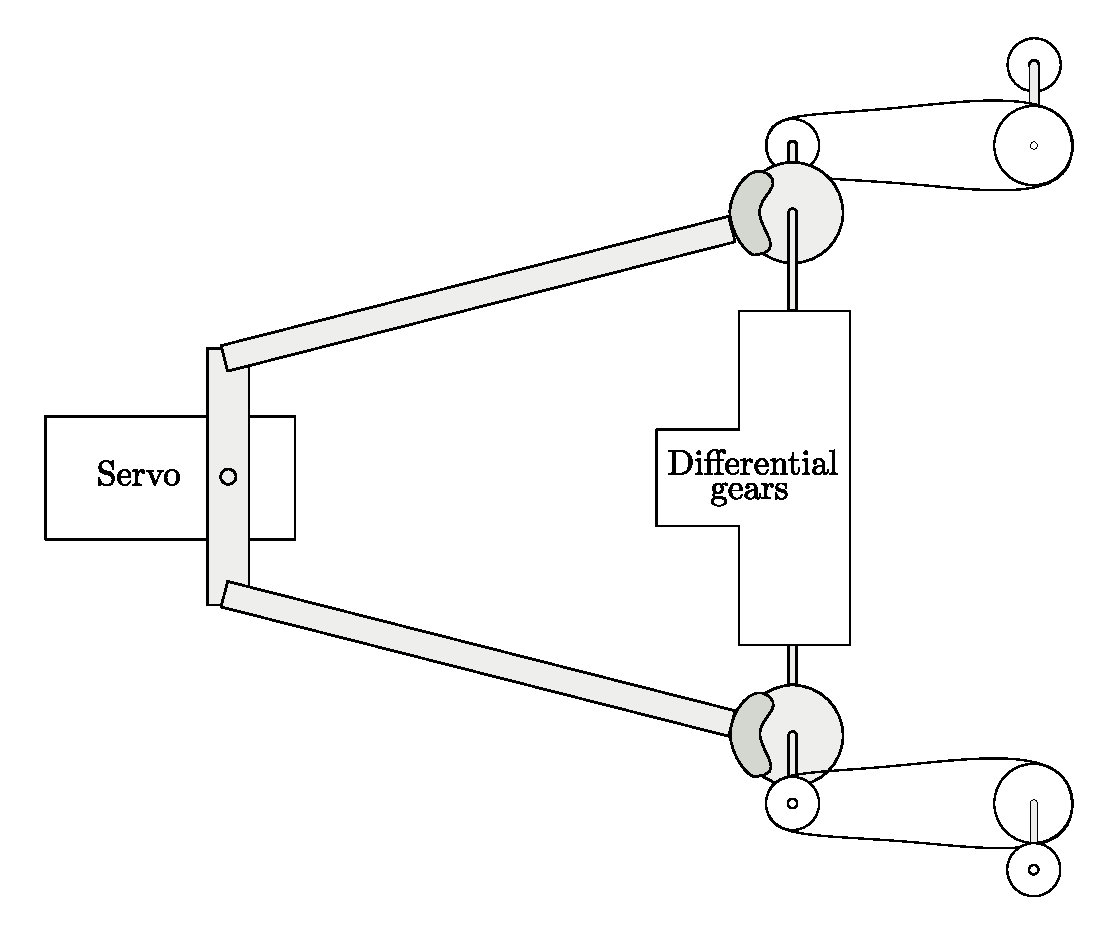
\includegraphics[scale=0.6]{figures/steeringMechanical.pdf}
 	\caption{Mechannical drawing of the steering}
 	\label{steeringMechanical}
 \end{figure}

Decription of how the vehicles steering is working

\subsection{Steering Parameters}
 To obtain a steering model everything in the system between the input and the output is black boxed. Second or first order, if it is second the black box should be expanded, if it is first there is no need because then we have all the parameters from the test.
 
 figure of the black box
 \begin{figure}[H]
 	\centering
 	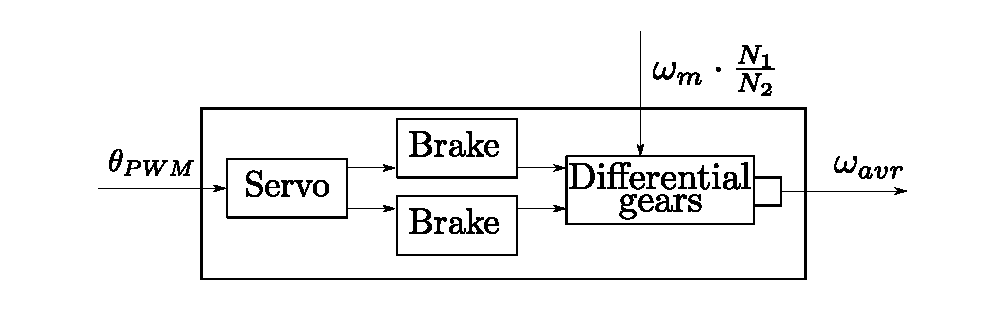
\includegraphics[scale=1]{figures/steeringDiagramBlackBox.pdf}
 	\caption{A diagram showing the black box}
 	\label{steeringDiagramBlackBox}
 \end{figure}
 
 appendix
 
setting up the first order system blabla. 
